\documentclass{article}
\usepackage{graphicx}
\usepackage{amsmath}
\usepackage[mathletters]{ucs}
\usepackage[utf8x]{inputenc}
\usepackage{listings}
\lstnewenvironment{code}{\lstset{language=Haskell,basicstyle=\small\ttfamily}}{}
\setlength{\parindent}{0pt}
\setlength{\parskip}{6pt plus 2pt minus 1pt}

\usepackage{pgf, tikz}
\usetikzlibrary{shapes}
\usetikzlibrary{shapes.multipart}
\usetikzlibrary{arrows}


\usepackage{array}
% This is needed because raggedright in table elements redefines \\:
\newcommand{\PreserveBackslash}[1]{\let\temp=\\#1\let\\=\temp}
\let\PBS=\PreserveBackslash



%\newcommand{\solution}[1] {}
\newcommand{\solution}[1] {\textbf{Solutions:}\\ #1}

% \setcounter{secnumdepth}{0}

\begin{document}
\newcommand{\examtime}{14:00, Thursday April 28th, 2011}
\newcommand{\points}[1]{\marginpar{\bf #1 points}}
\noindent
\begin{tabular}{lr}
CHALMERS TEKNISKA H\"OGSKOLA &\examtime{}.\\
Dept. of Computer Science and Engineering & Programming Paradigms\\
John Hughes                  & DAT120 / DIT330(GU) \\
\end{tabular}

\vspace{2.5cm} \noindent
\begin{center} {\LARGE
Exam in Programming Paradigms}
\end{center}

\vspace{1.5cm}

\noindent
\examtime{}.\\
\begin{tabular}{lllc}
\textbf{Lecturer:} &  John Hughes  & & (Examiner)\\
\textbf{Lecturer:} & Richard Bubel & tel 073 965 7355 & \\ 
\end{tabular}
\vspace{1cm}

\noindent
Permitted aids:\\
English-Swedish or English-other language dictionary.

There are five ordinary questions, one on each paradigm, worth 12
points each for a total of 60 points. 24 points is required to pass
(grade 3), 36 points is required for grade 4, and 48 points is
required for grade 5.\\
Grades for GU: 24~points is required for G and 48~points is required
for VG\\

Sheets are two-sided.

%\newcommand{\comment}[1]{}
\newcommand{\comment}[1]{\marginpar{#1}}

\newpage
This page is left blank intentionally.
\hfill
\newpage

\section{Functional Programming [12 points]}
\begin{enumerate}
\item {\bf $\lambda$-expressions}
Simplify the following $\lambda$-expressions as far as possible using $\beta$-reductions, showing the $\lambda$-expression obtained after each step.
\points{2}
\begin{enumerate}
\item
$(\lambda x.\lambda y.\lambda z.x~z~(y~z))~(\lambda a.\lambda b.b)~(\lambda c.\lambda d.d)$
\item
$(\lambda x.x~x)~(\lambda x.x~x)$
\end{enumerate}
\item {\bf Lists}.  In Haskell, the \verb!reverse! function reverses a
  list, so for example \verb!reverse [2,4]! is
  \verb![4,2]!.  What then is the value of this Haskell expression?
\begin{verbatim}
let xs = [1,2,3]
    ys = reverse xs
    zs = reverse xs
in (xs==ys, xs==zs, ys==zs)
\end{verbatim}
\points{1}
\item {\bf Lisp vs Haskell}.  Give two important differences between
 the Lisp and Haskell programming languages. \points{1}
\item {\bf Higher-order functions}
\begin{enumerate}
\item Simplify the expression \verb!foldr (+) z [a,b,c]! to one only
  involving variables and \verb!+!. Make sure the result you give is
  unambiguous: in particular, do not assume that \verb!+! is
  associative.
\points{1}
\item Replace \dots{} in this definition
\begin{verbatim}
numVal = foldl (...) 0
\end{verbatim}
by a $\lambda$-expression to make \verb!numVal! convert lists of decimal digits to the value of the number they represent. For example,
\begin{verbatim}
numVal [1,2,3] == 123
numVal [4,0,4,8] == 4048
\end{verbatim}
\points{1}
\end{enumerate}
\item {\bf take and drop}
Study the following Haskell definitions:
\begin{verbatim}
take 0 xs = []
take n [] = []
take n (x:xs) = x:take (n-1) xs

drop 0 xs = xs
drop n [] = []
drop n (x:xs) = drop (n-1) xs
\end{verbatim}
\begin{enumerate}
\item
What is the value of \verb!let s="hello" in (take 3 s, drop 3 s)!?
\points{1}
\item
Write a QuickCheck property relating \verb!take!, \verb!drop!, and \verb!++!.
\points{1}
\item
Which of the functions \verb!take! and \verb!drop! allocate memory when they are called?
\begin{enumerate}
\item \verb!take!
\item \verb!drop!
\item both
\end{enumerate}
\points{1}
\item
An important compiler optimization used by functional language
compilers is applicable to one of these definitions. Which function
can be optimised, what is the optimisation, and what is its effect?
\points{1}
\item
Rewrite the {\em other} function so that the same optimisation is
applicable. {\em Hint:} you may need to define an auxiliary function
of your own, and make use of the \verb!reverse! function in your
solution.  \points{2}
\end{enumerate}

\end{enumerate}


\newpage
\section{Concurrency Oriented Programming [12 points]}

\begin{enumerate}
\item
State two important differences between message passing in Erlang and
message passing in CSP.
\points{1}

\item
Study the following code, which starts a server managing an integer value:
\begin{verbatim}
server() ->
    spawn(fun() -> server(0) end).

server(N) ->
    receive
        {read,Pid} ->
            Pid ! {self(),N},
            server(N);
        {write,New} ->
            server(New)
    end.
\end{verbatim}
Write the following functions for use in clients of the server:
\begin{enumerate}
\item
\verb!read(ServerPid)!, which returns the value \verb!N! currently managed by the server,
\points{1}
\item
\verb!write(ServerPid,New)!, which updates the value currently managed by the server to \verb!New!.
\points{1}
\end{enumerate}

\item
What value(s) can the following function return:
\begin{verbatim}
test() ->
    Server = server(),
    spawn(fun() -> write(Server,read(Server)+1) end),
    spawn(fun() -> write(Server,read(Server)+1) end),
    read(Server).
\end{verbatim}
\points{1}

\item
Extend the server to handle two new requests, to {\em lock} and {\em
  unlock} the server, such that the next request serviced after a {\em
  lock} must be an {\em unlock} request from the same client. Define
the following functions for use in clients:
\begin{enumerate}
\item
\verb!lock(ServerPid)!, which returns the value \verb!N! currently
managed by the server, and prevents any other request from being
serviced until
\points{1}
\item
\verb!unlock(ServerPid,New)!, which updates the value currently
managed by the server to \verb!New!, and permits other clients to use
the server again.
\points{1}
\end{enumerate}
Write the code which must be added to the \verb!server(N)! function to
handle these two new requests.
\points{2}
\item
Suppose clients and servers exchange requests as shown in the diagram
below, when a client requests a service from a server. (Note that we
did not follow this protocol in the code above).

\begin{center}
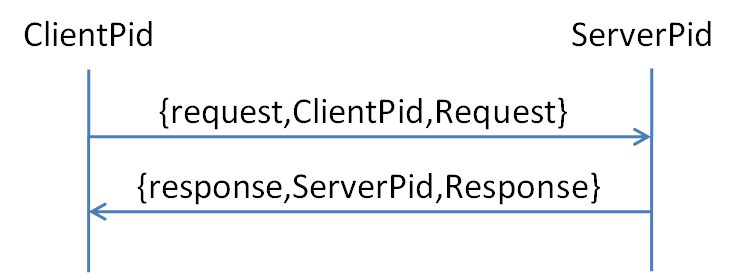
\includegraphics[width=10cm]{Diagram2.jpg}
\end{center}

A {\em load balancer} is a server which manages a number of other
servers, accepting requests from clients and forwarding them to
whichever managed server is currently free, and forwarding responses
from managed servers back to the correct client. This enables many
requests to be serviced in parallel, increasing the throughput of the
system.  Write the body of a load balancer process in Erlang, in the
form of a recursive function \verb!balance(Free,Busy)!, where
\verb!Free!  is a list of pids of servers which are currently idle,
and \verb!Busy!  is a list of pairs \verb!{ServerPid,ClientPid}!,
where \verb!ServerPid! is currently busy performing a request for
\verb!ClientPid!. You may operate on this list of pairs using the
functions
\begin{itemize}
\item
\verb!add_pair(ServerPid,ClientPid,List)! to add a pair to the list;
\verb!add_pair(S,C,L) -> [{S,C}|L]!. 
\item
\verb!lookup(ServerPid,List)! to find the associated \verb!ClientPid!
in the list; for example \verb!lookup(b,[{a,1},{b,2}]) == 2!.
\item
\verb!delete_pair(ServerPid,List)! to delete \verb!ServerPid! and its
associated client pid from the list; for example\\
\verb!delete_pair(b,[{a,1},{b,2}]) == [{a,1}]!. 
\end{itemize}
Make sure that your code communicates with both the managed servers
and the clients using messages matching those in the diagram.
\points{4}


\end{enumerate}

\newpage



\section{Basic Imperative and Object-Oriented Concepts [12 points]}
\lstset{language=Java, columns=flexible}

\begin{enumerate}
\item Let \lstinline!A! be a class with an integer typed attribute
  \lstinline!a!.
\begin{lstlisting}[language=Java, columns=flexible]
class A {  int a;  }
\end{lstlisting}

and the following program fragment
\begin{lstlisting}[language=Java, columns=flexible] 
A x; A y;
...
// x and y point to different objects
x.a = 1;
y.a = 2;

x = y;

x.a = 3;
y.a = 4;
      
x.a = x.a + y.a;   (*)
\end{lstlisting}
where the program variables \lstinline!x! and \lstinline!y! refer
initially to different objects.

Give the values of expression \lstinline!x.a! and expression
\lstinline!y.a! after execution of line~\lstinline!(*)! if the
assignment operator of the programming language is realised using
\begin{enumerate}
  \item copy semantics 
  \item reference semantics 
\end{enumerate}
\points{2}
\item Consider an imperative programming language \textsf{IMP} that
  allocates activation records \emph{statically} (i.e., at
  compile-time) for each method (function).
  \begin{enumerate}
  \item What is the problem with recursion in such a setting?\points{1}
  \item Assume \textsf{IMP} is able to allocate an arbitrary number of
    activation records per method at compile-time. Further, put
    yourself in the role of a developer who is implementing a compiler
    for \textsf{IMP}. Your aim is to enable the programmer to use to
    some extent recursion. What must your compiler be able to
    determine to compile successfully a program that uses recursion?
    (If the compiler is not able to determine the property/-ies, it
    will reject the program.)\points{2}
 \end{enumerate}
\item Given the following program:
\begin{lstlisting}[language=Java, columns=flexible] 
int f(int a) {
  return a * 2;  // (*)
} 

int g(int b, int c) {
  if (b < c) {
    return g(c,b); 
  }
  int r = f(a-b);
  return r;
}
\end{lstlisting}

Consider the call 
\begin{center}
  \lstinline[language=Java, columns=flexible]{g(3,8)} 
\end{center}
Give the number of activation records on the stack resulting from the
above call just before returning from (*), i.e., directly after
assigning the return value, but before popping the last activation
record from the stack. Give also the last two activation records on
top of the stack (the last allocated ones). State their order
explicitly and name all slots/components of the activation record and
their content explicitly. If a content is not yet defined use
'\texttt{?}' as value. \points{3}
\item Consider the following program
\begin{lstlisting}[language=Java, columns=flexible] 
void f(by-?? int a, by-?? int b, by-?? int c) {
  a = a + a;
  b = a + b + c;
  c = c + 15;
}

 ..
 int i, j;
 i = 1; 
 j = 5;
 f(i+1, j, j); //(*)
\end{lstlisting}

What are the values of the variables \lstinline!i! and \lstinline!j!
at (*) after the method \lstinline!f! returns if
\begin{enumerate}
  \item all parameters are passed \emph{by-copy}
  \item parameter \lstinline!a! is passed \emph{by-copy} and
    the parameters \lstinline!b! and \lstinline!c! \emph{by-reference}
  \item the parameters \lstinline!a! and \lstinline!b! are passed
    \emph{by-copy} and parameter \lstinline!c! \emph{by-value-result}.
  \item parameter \lstinline!a! is passed \emph{by-name}, parameter
    \lstinline!b! is passed \emph{by-reference} and parameter
    \lstinline!c! is passed \emph{by-copy}.
\end{enumerate} \points{4}
\end{enumerate}

\solution{
\begin{enumerate}
\item
  \begin{enumerate}   
  \item \lstinline!x.a!: 7 \quad  \lstinline!y.a!: 4
  \item \lstinline!x.a!: 8  \quad \lstinline!y.a!: 8
  \end{enumerate}
\item 
  \begin{enumerate}
  \item the problem is that (in general) the recursion depth cannot be
    determined a priori. Consequently, recursive calls would cause the
    values in living activation records to be overwritten.
  \item the maximum recursion depth for each method
  \end{enumerate}
\item 3 activation records are on the stack; the last two ones
  $A_1$,$A_2$ where $A_2$ is the one on top of the stack are defined
  as follows: $A_1=(8,3,?,\text{ref to}~A_{0} , ?)$ (first two parameters,
  third local variable, fourth reference to first activation record,
  fifth return value), $A_2=(5, \text{ref to}~A_1, 10)$  
\item\hfill\\
  \begin{tabular}{lcc}
    & \lstinline!i! & \lstinline!j! \\ \hline
   (a) &  1 & 5 \\
   (b) & 1 & 29 \\
   (c) & 1 & 20 \\
   (d) & 1 & 15 \\
  \end{tabular}

  
\end{enumerate}
}

\newpage

\section{Object-Oriented Programming [12 points]}

\begin{enumerate}
\item Describe briefly in not more than three to four short sentences,
  why data encapsulation is desirable.\points{2}
\item Repeated inheritance is when a class serves as ancestor
  repeatedly through different inheritance paths. Name two semantics
  (ways to implement/realize) of repeated inheritance. \points{1}
\item One motivation for allowing repeated inheritance is to achieve
  better and more flexible code reuse than achievable with single
  inheritance. Name two alternatives to repeated inheritance aiming to
  provide better code reuse avoiding some of the disadvantages of
  repeated inheritance. \points{2}
\item Given the following class
  hierarchy \\
\begin{center}

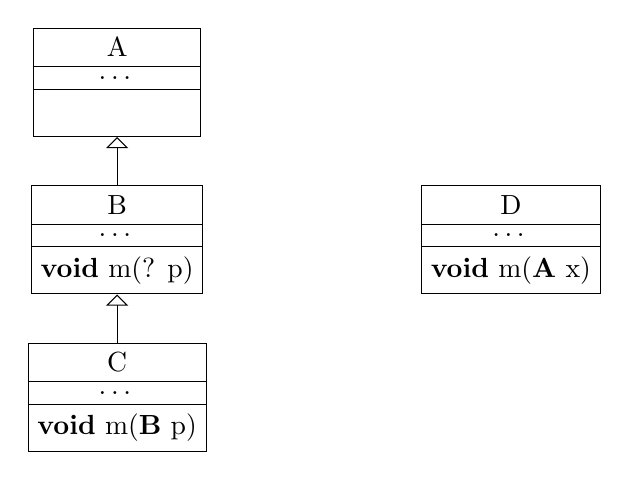
\begin{tikzpicture}
\node[draw, 
   rectangle split, 
   rectangle split parts=3, 
   minimum width=2cm] (A) at (5,4) 
  {A 
     \nodepart{second} \ldots 
     \nodepart{third} \phantom{\textbf{void} h(A x)}};
\node[draw, 
   rectangle split, 
   rectangle split parts=3, 
   minimum width=2cm] (B) at (5,2) 
  {B 
     \nodepart{second} \ldots 
     \nodepart{third} \textbf{void} m(? p)};
\node[draw, 
   rectangle split, 
   rectangle split parts=3, 
   minimum width=2cm] (C) at (5,0) 
  {C 
    \nodepart{second} \ldots 
    \nodepart{third} \textbf{void} m(\textbf{B} p)};   

\node[draw, 
   rectangle split, 
   rectangle split parts=3, 
   minimum width=2cm] (D) at (10,2) 
  {D 
     \nodepart{second} \ldots 
     \nodepart{third} \textbf{void} m(\textbf{A} x)};

\draw[open triangle 90-] (A) -- (B);
\draw[open triangle 90-] (B) -- (C);
\end{tikzpicture}
\end{center}
defining all available classes. Note: Class \lstinline!A! does not
define any method.
Give for each of the following overriding semantics (for arguments):
\begin{enumerate}
  \item co-variance,
  \item contra-variance and
  \item invariance
\end{enumerate}
\emph{all} possible argument types for method \lstinline!m! in class
\lstinline!B! such that \lstinline!m! is overridden by the method
\lstinline!m! declared in class \lstinline!C!.  \points{3}\newpage
\item Given the following class hierarchy:\\
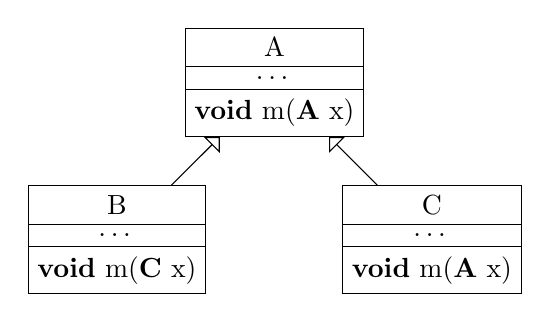
\begin{tikzpicture}
\node[draw, 
   rectangle split, 
   rectangle split parts=3, 
   minimum width=2cm] (A) at (5,4) 
  {   A 
     \nodepart{second} \ldots 
     \nodepart{third} \textbf{void} m(\textbf{A} x)};
\node[draw, 
   rectangle split, 
   rectangle split parts=3, 
   minimum width=2cm] (B) at (3,2) 
  {B 
     \nodepart{second} \ldots 
     \nodepart{third} \textbf{void} m(\textbf{C} x)
  };
 \node[draw, 
    rectangle split, 
    rectangle split parts=3, 
    minimum width=2cm] (C) at (7,2) 
  {C 
    \nodepart{second} \ldots 
    \nodepart{third} \textbf{void} m(\textbf{A} x)};   
\draw[open triangle 90-] (A) -- (B);
\draw[open triangle 90-] (A) -- (C);
\end{tikzpicture}

Overriding semantics for methods is such that the method \lstinline!m!
of class \lstinline!B! as well as the method \lstinline!m! of class
\lstinline!C! override the method \lstinline!m! defined in class
\lstinline!A!. 

In addition there is a method \lstinline!g! 
\begin{lstlisting}[language=Java, columns=flexible]
void g(A x, B y) {
   x.m(y);
}
\end{lstlisting}

Which of the three implementations of method \lstinline!m! is invoked by
\lstinline!g! if
\begin{enumerate}
\item the programming language uses \emph{single-dynamic dispatch} and
  the call statement is
 \begin{enumerate}
    \item \lstinline!g(new B(), new B());!
    \item \lstinline!g(new B(), new C());!
  \end{enumerate}
  \item the programming language uses \emph{multi-dynamic dispatch}
    and the call statement is
 \begin{enumerate}
    \item \lstinline!g(new B(), new B());!
    \item \lstinline!g(new B(), new C());!
    \end{enumerate}
\end{enumerate}\points{2}
\item Which of the following statements are true\\
    \begin{tabular}{|p{6cm}|c|c|}\hline
      & True & False \\ \hline
      a) F\# runs on the \textsf{.net} virtual machine, but cannot use the
      normal libraries as it is a functional language, while the normal
      libraries on \textsf{.net} are object-oriented. & & \\\hline
      b) In F\# declaring variables mutable or as reference cells has
      the same meaning. & & \\\hline
      c) F\#-Expressions are side-effect free. & & \\\hline
      d) Smalltalk has no distinguished loop statement instead loops
      are realized as methods invoked on block closures.  & & \\\hline
   \end{tabular}\\
   For your answer draw that table but refer to the statements by a),
   b) etc. instead of writing them again. Wrong answers lead to a
   reduction of points, a negative result does not carry over to other
   sub-assignments. \points{2}
\end{enumerate}

\solution{
\begin{enumerate}
\item Hides internal datastructures, providing access to clients only
  via methods. Allows to change internal datastructures (e.g., by
  better performing or reliable ones) without requiring changes on
  client side.
\item \emph{Replicated Inheritance}, \emph{Shared (diamond)
    Inheritance}
\item \emph{Mix-ins}, \emph{Traits} (attention \emph{Interfaces}
  provide complex subtyping, but not code reuse)
\item 
    \begin{enumerate}
      \item A, B
      \item B, C
      \item B
    \end{enumerate}
\item 
    \begin{enumerate}
    \item 
    \begin{enumerate}
    \item method \lstinline!m! as defined in class \lstinline!A!
    \item method \lstinline!m! as defined in class \lstinline!A!
  \end{enumerate}
    \item 
    \begin{enumerate}
    \item method \lstinline!m! as defined in class \lstinline!A!
    \item method \lstinline!m! as defined in class \lstinline!B!
    \end{enumerate}
    \end{enumerate}
\item
      \begin{tabular}{|p{6cm}|c|c|}\hline
      & True & False \\ \hline
      a) F\# runs on the \textsf{.net} virtual machine, but cannot use the
      normal libraries as it is a functional language, while the normal
      libraries on \textsf{.net} are object-oriented. & & X \\\hline
      b) Declaring variables mutable or as reference cell in F\# has
      the same meaning. & & X \\\hline
      c) F\#-Expressions are side-effect free. & & X \\\hline
      d) Smalltalk has no distinguished loop statement instead loops
      are realized as methods invoked on block closures.  & X & \\\hline
   \end{tabular}\\

\end{enumerate}
}

\newpage


\section{Logic Programming [12 points]}

\begin{enumerate}
\item
Given the three clauses
\begin{enumerate}
\item \verb!A || B!
\item \verb!C || D!
\item \verb?!A || D?
\end{enumerate}
state {\em which two} of the clauses can be combined using a resolution step, and give the resulting clause.
\points{1}

\item
For each pair of terms below, state whether the terms can be unified,
and if so, give the variable bindings that result. For example,
\verb!X! and \verb!2! {\em can} be unified, and the result is
\verb!X=2!.
\begin{enumerate}
\item \verb![X|Xs]! and \verb![1,2,3]!
\item \verb![X|Xs]! and \verb![]!
\item \verb!pair(A,y)! and \verb!pair(x,B)!
\item \verb!X! and \verb!Y!
\item \verb!pair(A,A)! and \verb!pair(B,C)!
\item \verb!pair(A,A)! and \verb!pair(b,c)!
\end{enumerate}
\points{3}

\item
Study the following Prolog program:
\begin{verbatim}
father(jack,robert).
father(robert,desmond).
father(robert,william).
mother(catherine,robert).
mother(mary,desmond).
mother(mary,william).
\end{verbatim}
What solutions will Prolog find for the following goals?
\begin{enumerate}
\item \verb!father(X,robert).!
\item \verb!father(robert,X).!
\end{enumerate}
\points{2}

\item
Extend the program above by defining a predicate \verb!parents(X,Y,Z)!
which holds if \verb!X! and \verb!Y! are the parents of \verb!Z!, and
\verb!X! is the father.
\points{1}

\item 
What solutions would Prolog find for the query \verb!parents(X,Y,Z)!?
\points{1}

\item
Study the following Prolog definitions:
\begin{verbatim}
append([],Ys,Ys).
append([X|Xs],Ys,[X|Zs]) :- append(Xs,Ys,Zs).
mystery([],[]).
mystery([X|Xs],Ys) :- mystery(Xs,Zs), append(Zs,[X],Ys).
\end{verbatim}
What solutions will Prolog find for the queries
\begin{enumerate}
\item \verb!mystery([1,2,3],X).!
\item \verb!mystery(X,[1,2,3]).!
\end{enumerate}
\points{2}

\item
One of the \verb!mystery! queries falls into an infinite loop after
printing the solutions. Which one?
\points{1}


\item
Rewrite the definition of \verb!mystery! to find the same solutions,
but so that neither of these queries falls into an infinite loop.
\points{1}

\end{enumerate}


\end{document}
